\section*{Разработка интерфейса}
\addcontentsline{toc}{section}{Разработка интерфейса}

Для любой программы интерфейс является одной из наиболее важных составляющих.
Ведь именно он определяет, как приложение будет взаимодействовать с другими
программами и своими пользователями. Таким образом, можно ввести следующую
классификацию интерфейсов:

\setlist{nolistsep}
\begin{enumerate}
    \item программные,
    \item графические,
    \item интерфейсы командной строки.
\end{enumerate}

Несмотря на то, что эти интерфейсы имеют между собой мало общего, к ним 
предъявляется ряд общих требований:

\begin{enumerate}
    \item функциональность -- интерфейс должен отвечать всем требованиям пользователя и соответствовать его задачам,
    \item логичность -- интерфейс должен быть логичным и запоминающимся, чтобы взаимодействие пользователя
        с программой было как можно более простым и удобным,
    \item защищенность -- интерфейс должен быть спроектирован таким образом, чтобы у пользователя не было
        возможности совершить ошибку.
\end{enumerate}

После определения общих требований к любому интерфейсу, стоит рассмотреть перечисленные выше
интерфейсы отдельно.

\subsection*{Программные интерфейсы}
\addcontentsline{toc}{subsection}{Программные интерфейсы}

К программным интерфейсам можно причислить любой интерфейс, который предназначен для
использования разрабатываемой программы внешними приложениями. Обычно, в зависимости от
используемых технологий, это набор классов, функций или методов, которые используются
внешними программами. В случае данного приложения в качестве интерфейса взаимодействия
было решено использовать веб-технологии. Это означает, что приложение будет взаимодействовать
с любыми своими пользователями через протокол HTTP.
Таким образом, программный интерфейс приложения будет представлять из себя набор HTTP-методов.

В протоколе HTTP есть несколько видов методов, из которых приложением будут использоваться следующие:

\begin{enumerate}
    \item GET -- это методы, которые запрашивают данные, они не предназначены для их записи,
    \item POST -- это методы, которые используются и для записи данных, и для их получения.
\end{enumerate}

Говоря об HTTP интерфейсах, стоит отметить, что есть несколько различных подходов к проектированию
подобных интерфейсов. Одним из наиболее общепринятых подходов является так называемый REST.
Это можно перевести как Represental State Transfer\cite{REST}. Данная архитектура предлагает
наложить на приложение ряд следующих ограничений:

\begin{enumerate}
    \item модель клиент-сервер -- означает, что вся логика должна выполняться на удаленном сервере,
    а клиентское приложение должно исключительно предоставлять и получать данные,
    \item отсутствие состояния -- сервер получает из запроса всю необходимую информацию и не хранит
    никакую информацию о сессии клиентов,
    \item кэширование -- сервер сохраняет наиболее частые ответы, что позволяет не выполнять
    лишние запросы к базе данных и соответствующие вычисления, а сразу вернуть результат,
    \item единообразие интерфейса,
    \item слои -- сокрытие основного сервера за промежуточными. Например, без каких-либо
    изменений для пользователя можно внедрить между ним и сервером промежуточный сервер, который
    предназначен для хранения и отдачи хэшированных данных. В случае отсутствия этих данных
    хэширующий сервер перенаправляет запрос исходному серверу.
\end{enumerate}

Такой подход позволяет добиться лучшей производительности за счет отсутствия состояний между
вызовами и кэширования, а архитектура становится более расширяемой из-за требований
единообразия и использования слоев.

\subsection*{Графические интерфейсы}
\addcontentsline{toc}{subsection}{Графические интерфейсы}

Графические интерфейсы -- это наиболее востребованные интерфейсы в современном мире, потому
что пользователям намного более удобно пользоваться интерфейсами, у которых среди
средств донесения информации есть не только текст. 

И, пожалуй, самый популярный вид графических приложений -- это веб-сайты.
Они получили такую популярность из-за своей универсальности: пользователь
может открыть приложение на любом устройстве, на котором есть доступ в интернет
и веб-браузер, в то время как любое другое приложение потребует установки
на устройство пользователя. С другой стороны, веб-сайты очень удобны для
разработчиков. Намного более выгодно разработать одно веб-приложение, чем
создавать и поддерживать несколько программ для разных платформ.

Обычно разработку веб-приложения можно разделить на две части:
<<фронтенд>> и <<бэкенд>>.

<<Фронтенд>> -- это та часть приложения, которая исполняется в браузере пользователя.
Для написания веб-сайтов используются язык разметки HTML, язык описания стилей CSS и интерпретируемый
язык программирования JavaScript.

Опишем роль каждого языка в веб-приложении:
\begin{enumerate}
    \item HTML -- это каркас всего приложения, который определяет, какие элементы будут использоваться и
    где они будут располагаться,
    \item CSS определяет, как будут выглядеть элементы приложения. Сюда входят, например, внешний вид кнопок
    или вид шрифта отображаемого текста,
    \item JavaScript -- это интерпретируемый язык программирования, основная область применения которого заключается
    в придании интерактивности веб-страницам. Например, динамическую загрузку данных в таблицу можно реализовать только
    через JavaScript. 
    
\end{enumerate}

<<Бэкендом>> обычно называют ту часть приложения, которая стоит за <<фронтендом>>. В основном это
та программа, которая предоставляет данные, выполняет их хранение и агрегацию. Другими словами,
<<бэкенд>> реализует всю <<бизнес-логику>>, в то время как <<фронтент>> нужен для предоставления
пользователям доступа к приложению. Более подробно об этом будет рассказано далее.

\subsection*{Интерфейсы командной строки}
\addcontentsline{toc}{subsection}{Интерфейсы командной строки}

Интерфейсы командной строки, в отличии от графических и программных интерфейсов, представляют
наименее популярную группу приложений. Но, несмотря на это, они являются
незаменимыми. Главное преимущество приложений командной строки заключается в том, что
ими могут пользоваться в равной степени эффективно человек, и программа. Таким образом,
интерфейсы командной строки являются сочетанием программных и графических интерфейсов:
с одной стороны ими с определенной степенью удобства может пользоваться человек, а с другой
стороны без каких-либо трудностей они могут использоваться для взаимодействия между
приложениями. Также стоит отметить, что приложениям командной строки не нужен какой-либо
графический интерфейс, только окно терминала.

Для того, чтобы заниматься непосредственным проектированием интерфейсов, необходимо
понять задачу, которые они будут решать.

\subsection*{Постановка задачи}
\addcontentsline{toc}{subsection}{Постановка задачи}

Необходимо разработать приложение, которое выполняет генерацию списков литературы
для учебных курсов в формате BibTeX. Для этого приложение должно иметь следующие функции:

\begin{enumerate}
    \item Поиск информации о книгах;
    \item Хранение и модификация информации о книгах;
    \item Создание и модификация данных об учебных курсах;
    \item Генерация списка литературы.
\end{enumerate}

\subsection*{Разработка программного интерфейса}
\addcontentsline{toc}{subsection}{Разработка программного интерфейса}

При рассмотрении программных интерфейсов была описана архитертура REST. Согласно
этой архитектуре каждый метод должен принимать в себя всю необходимую информацию
для выполнения запроса, а все методы должны быть унифицированы. Таким образом, для каждого
вида данных был реализован следующий набор методов:

\begin{itemize}
    \item add\%Имя таблицы\% -- POST запрос, содержащий данные для добавления в теле,
    \item get\%Имя таблицы\% -- GET запрос, получающий данные от приложения,
    \item prototype\%Имя таблицы\% -- GET запрос, получающий прототип JSON-файла для искомой таблицы.
\end{itemize}

Также были реализованы две дополнительных команды: report и migrate.

Первая получает данные, необходимые для однозначной идентификации требуемого списка литературы
и генерирует для этого списка литературы файл в формате BibTeX. 

Команда migrate выполняет копирование списка литературы с одного года на другой. Это необходимо для того,
чтобы облегчить работу пользователя, ведь обычно учебные программы слабо меняются от года к году.

\subsection*{Разработка интерфейса командной строки}
\addcontentsline{toc}{subsection}{Разработка интерфейса командной строки}

Как уже было сказано выше, для интерфейсов командной строки крайне важна автоматизируемость.
Это делает невозможным использование так называемого интерактивного ввода. Другими словами,
любое действие пользователя должно совершаться за один вызов приложения. В результате
было решено использовать следующий подход к проектированию интерфейса: для каждого вида данных,
с которыми будет работать приложение, будет реализована собственная команда. И для каждой такой
команды будет реализован набор подкоманд, выполняющих необходимые действия. В общем случае
команду приложения командной строки можно описать в следующем виде:

\begin{itemize}
    \item \%Имя таблицы\% prototype -- данный метод добавляет новый файл в файловую систему,
        который содержит в себе прототип для нужного вида данных. После чего пользователь
        должен заполнить этот прототип информацией, которую хочет добавить,
    \item \%Имя таблицы\% add -- сохраняет данные в приложение,
    \item \%Имя таблицы\% get -- позволяет получить данные из приложения, можно конфигурировать
        флагами.
\end{itemize}

Также отличительной чертой хорошего приложения командной строки является грамотно оформленная справка.
Рисунок ~\ref{ris:help_example} показывает результат выполнения команды help. 

\begin{figure}[h!]
    \center{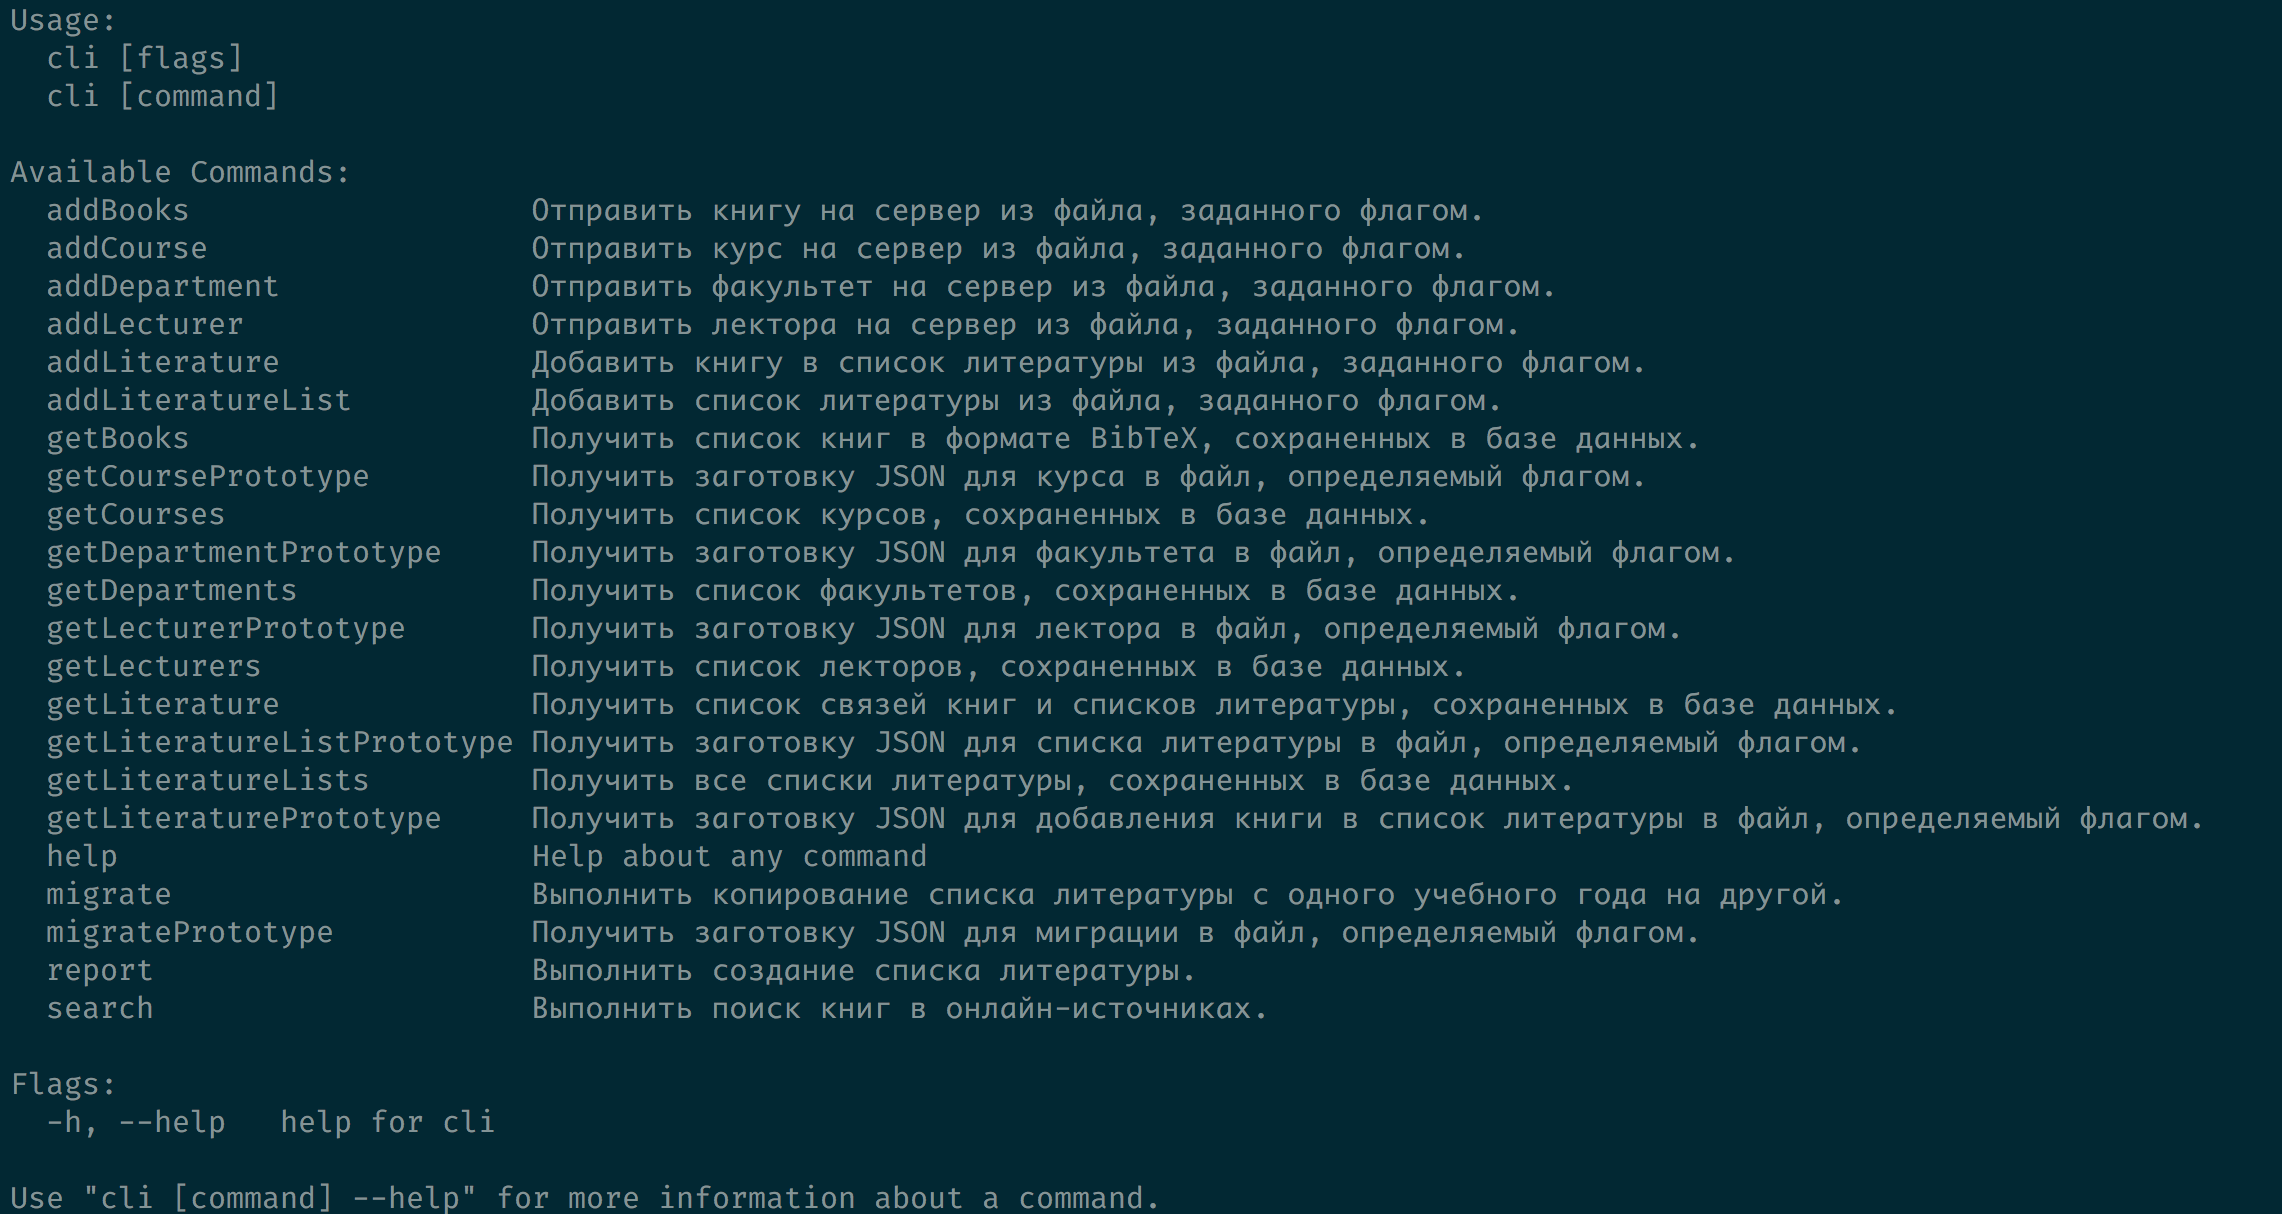
\includegraphics[width=1\linewidth]{help}}
    \caption{Пример работы команды help.}
    \label{ris:help_example}
\end{figure}

Также для каждой отдельной команды реализован
отдельный флаг --help, который показывает справку для конкретной команды, что можно видеть на рисунке 
~\ref{ris:help_book_example}. 

\begin{figure}[h!]
\center{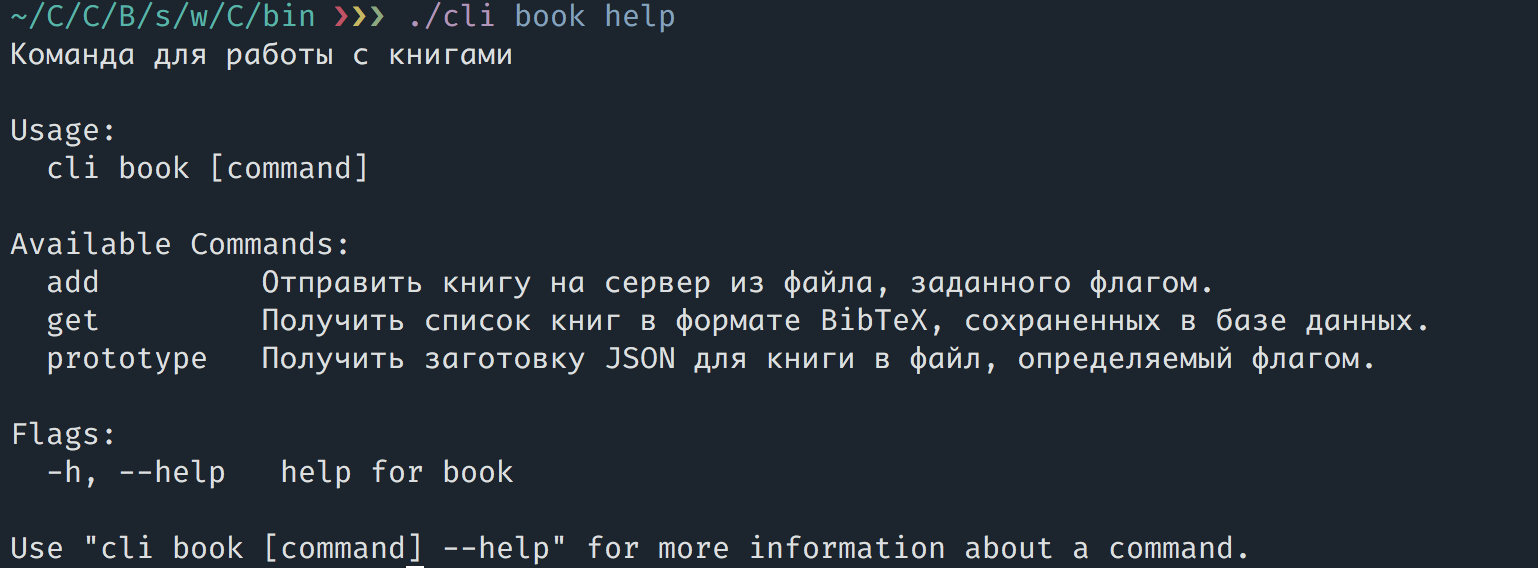
\includegraphics[width=1\linewidth]{help_book}}
\caption{Пример работы флага help для команды book}
\label{ris:help_book_example}
\end{figure}

\subsection*{Разработка графического интерфейса}
\addcontentsline{toc}{subsection}{Разработка графического интерфейса}

Как уже было сказано выше, графический интерфейс реализован в виде веб-сайта, написанного на языке TypeScript с 
использованием фреймворка Bootstrap.
Выбор фреймворка обусловлен тем, что он предоставляет продвинутый набор стилей и HTML-элементов, что позволяет 
легко и быстро настроить внешний вид веб-приложения.
В связи с тем, что единственный современный и поддерживаемый язык для написания веб-сайтов - это JavaScript, то 
из альтернатив ему можно использовать только языки, компилируемые в JavaScript. В частности, к таким языкам можно 
отнести язык TypeScript компании Microsoft и язык Kotlin, разрабатываемый компанией JetBrains, который имеет 
отдельный плагин для компиляции JS-код. К сожалению, Kotlin является очень молодым языком, который находится в 
активной разработке, так что было решено использовать TypeScript. Преимуществом данного языка является то, что 
он является надмножеством JavaScript. Это означает, что любой JavaScript код является абсолютно корректным. Также 
важно отметить, что TypeScript поддерживает важные аспекты объектно-ориентированого программирования: классы, 
инкапсуляцию(уточнить насчет остального). Но главным преимуществом этого языка является его строгая типизированность. 
Это облегчает разработку и позволяет писать более читаемый код по сравнению с JavaScript.

На рисунках ~\ref{ris:web_example_1} и ~\ref{ris:web_example_2} видно, приложение состоит из четырех логический частей. 

\begin{figure}[h!]
    \center{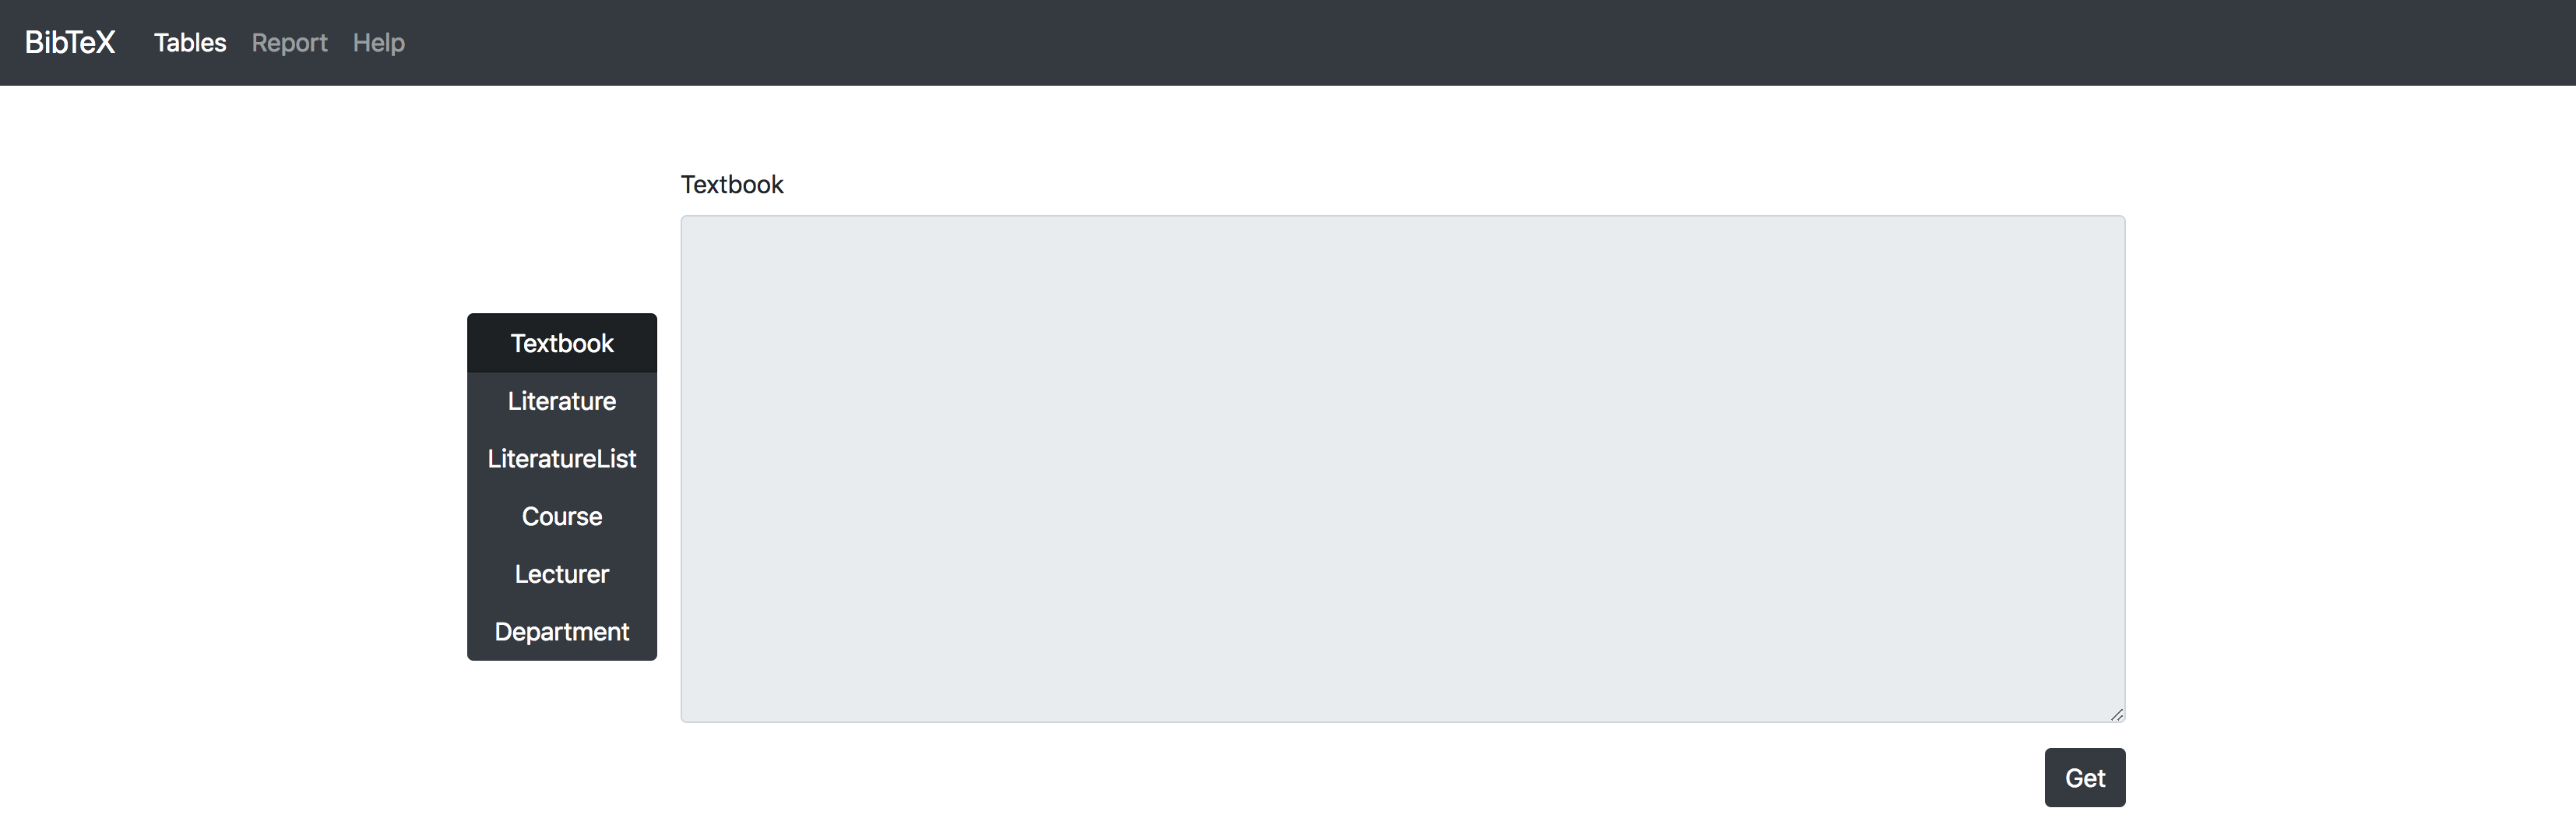
\includegraphics[width=0.8\linewidth]{web_example_1}}
    \caption{Верхняя часть веб-сайта}
    \label{ris:web_example_1}
\end{figure}

\begin{figure}[h!]
    \center{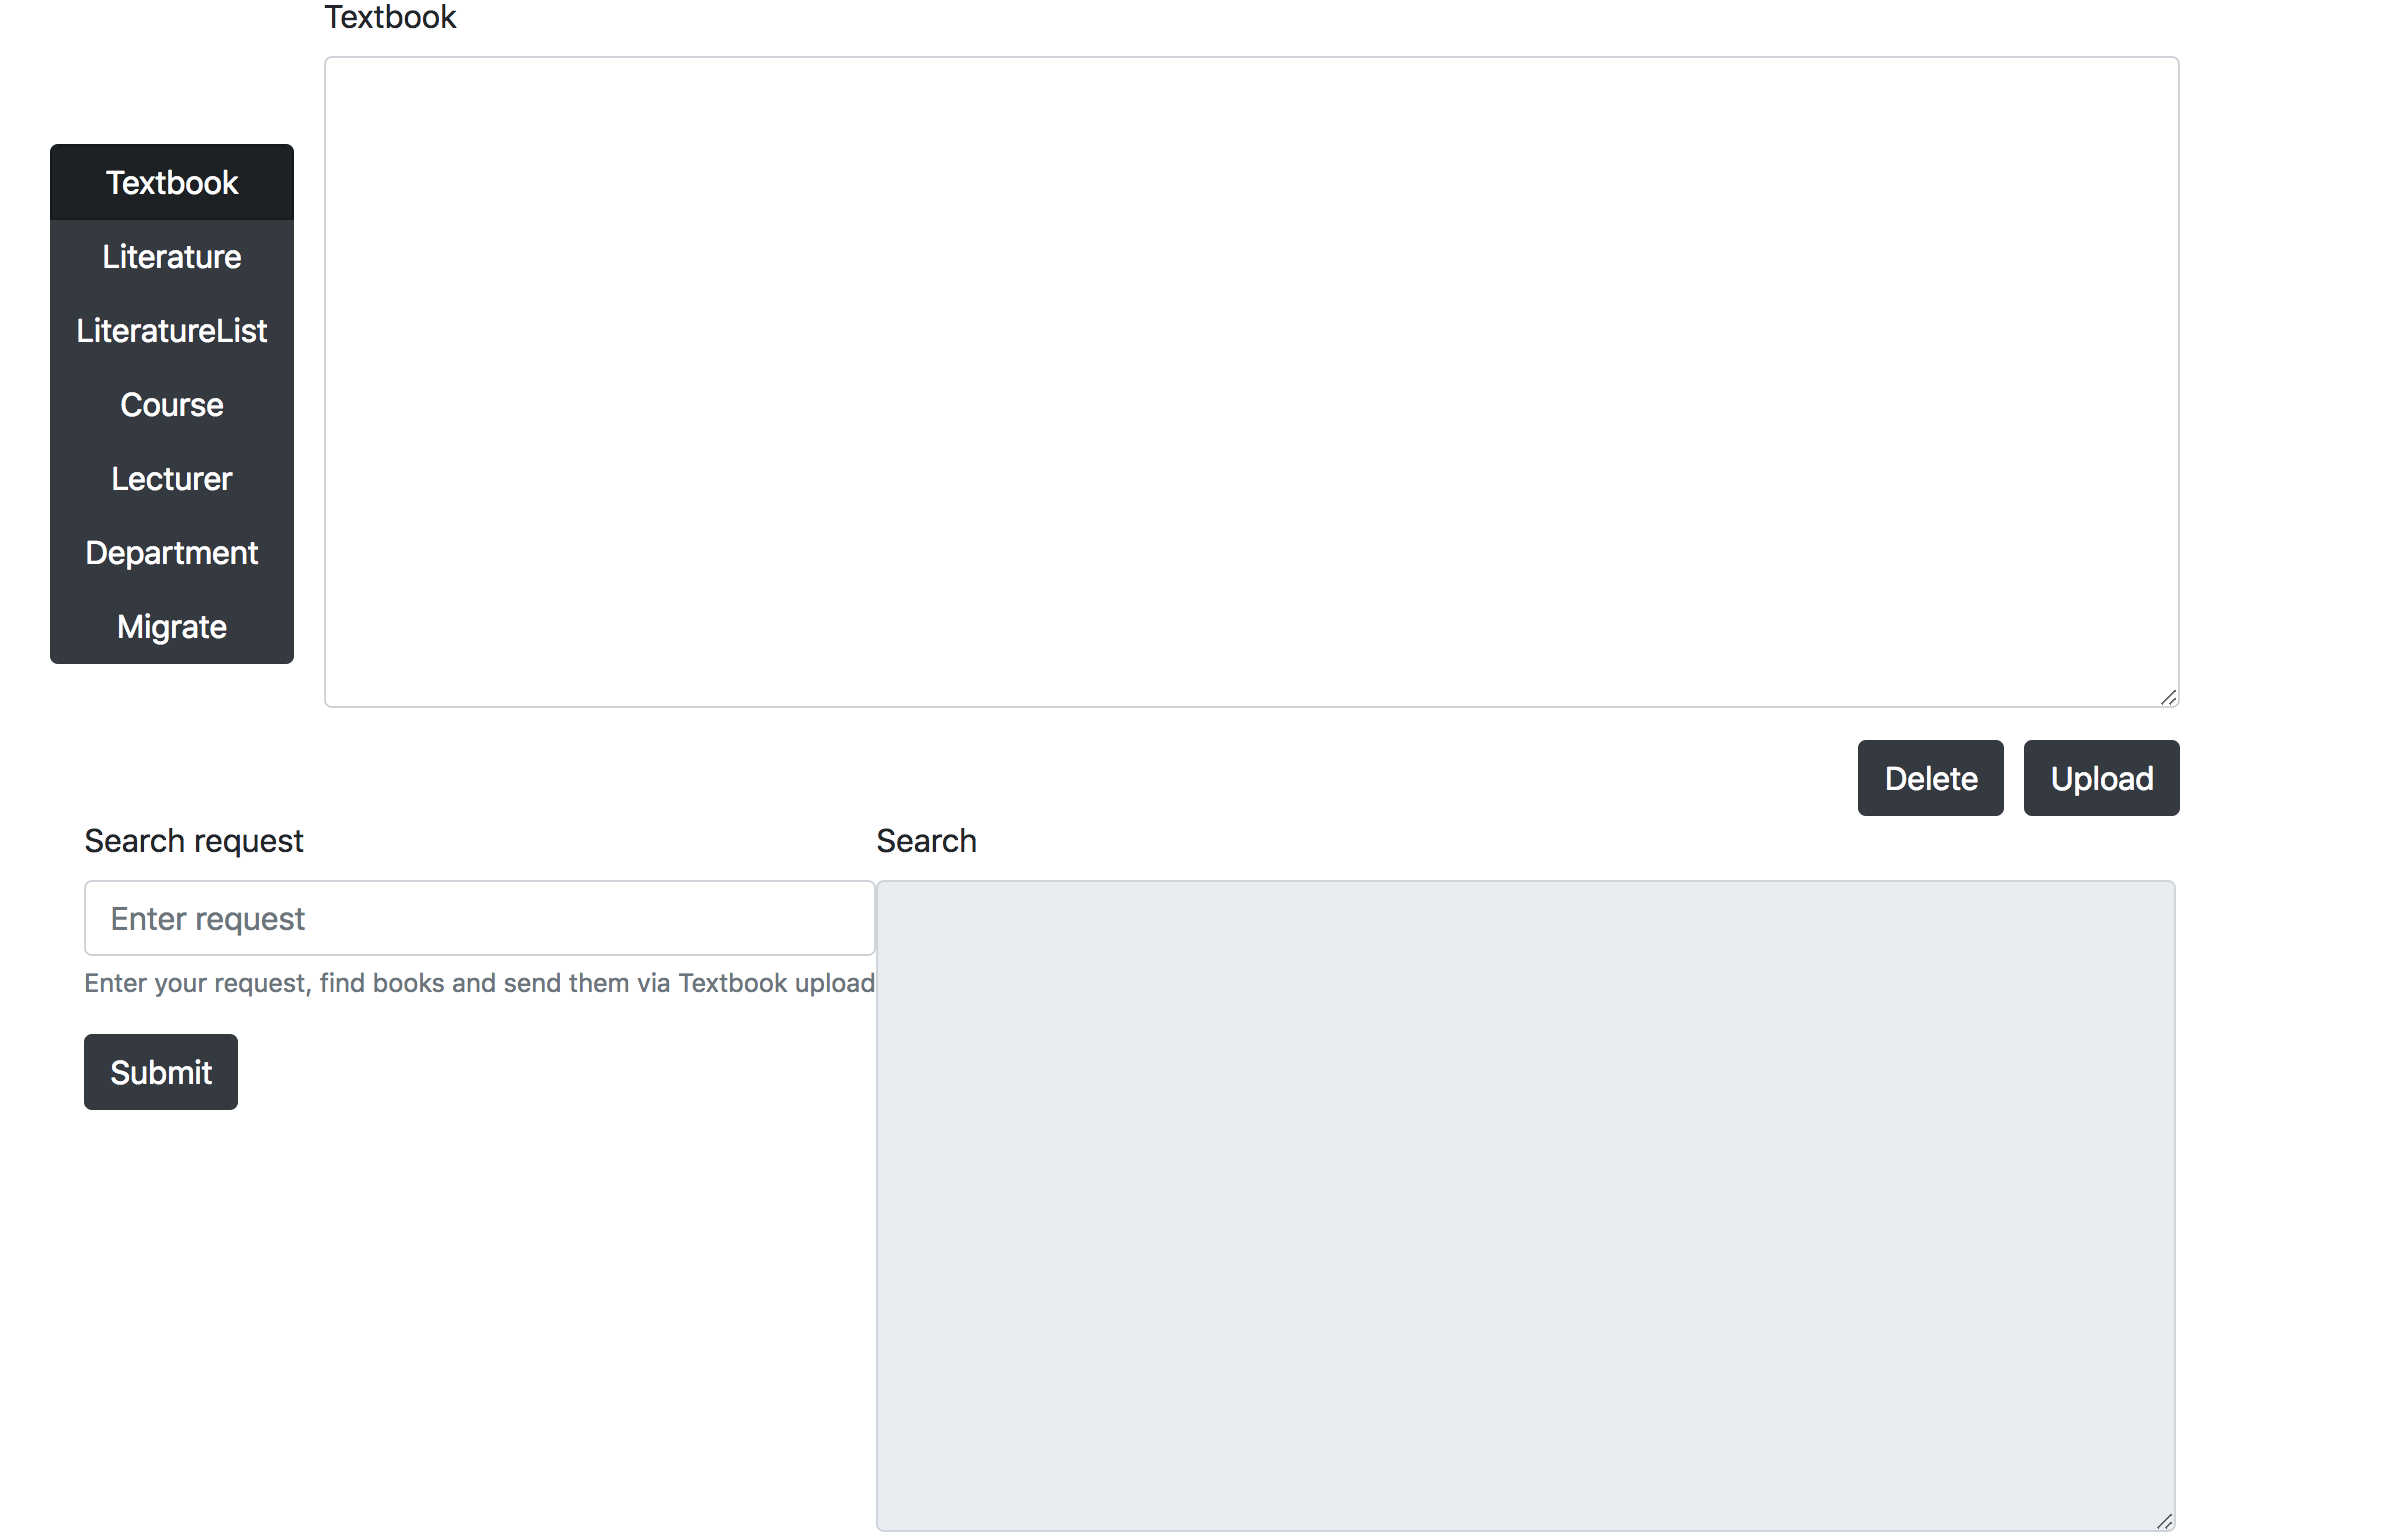
\includegraphics[width=0.8\linewidth]{web_example_2}}
    \caption{Нижняя часть веб-сайта}
    \label{ris:web_example_2}
\end{figure}

Первая - шапка сайта. Она содержит название 
приложения и ссылки на три страницы приложения: основную рабочую область, страницу генерации отчетов и страницу со 
справкой.

Вторая логическая часть - это большая недоступная для ввода область TextArea вместе с набором кнопок, 
отвечающих за переключение используемой таблицы. Эта часть нужна для получения данных, которые 
уже содержатся в базе данных для более удобного добавления новых записей в приложение.

Третья часть -- доступная для ввода область TextArea, в которую автоматически загружаются
JSON прототипы для текущего вида входных данных.

Заключительная область необходима для поиска необходимых книг в сервисе Google Books.
